%%% Research Diary - Entry
%%% Template by Mikhail Klassen, April 2013
%%% Modified by Pranav Sanghavi, May 2018
\documentclass[11pt,letterpaper]{article}

\newcommand{\workingDate}{\textsc{\today}}
\newcommand{\userName}{Pranav}

\usepackage{researchdiary_png}
\usepackage{rotating}

\begin{document}


{\Huge \today}\\[5mm] %Date of entry

\section{DSPIRA 2018 LNA Assemby}

We shall assemble our LNAs referring to the schematic and layout in Figures \ref{fig:schematic} and \ref{fig:layout} respectively. An assembly guide is given in \S 1.1

\subsection{Assembly}

Assemble all the surface mount passives first (Resistors, Capacitors and Inductors). Try to work from Left to right on the board, but also put on all components with the same value at once.

\begin{tabular}{l|cc}
  Component Label & Value  \\
  \hline
  L2 &  10 nH \\
  L1, L3, L4, L5, L6 & 100 nH \\
  C6 &  9.1 pF \\
  C1, C5 & 27 pF \\
  C15 & 6.8 pF \\
  C4 & 4700 pF \\
  C2, C3, C7, C8, C9, C10, C11, C12, C13, C14 & 330 pF \\
  R5 & 4.7k $ \Omega $  \\
  R2 & 27k $ \Omega $ \\
  R1 & 33k $ \Omega $ \\
  R3 & 50 $ \Omega $ \\
  R8 & 150 $ \Omega $ \\
  R4, R13 & 43 $ \Omega $ \\
  R6 & 17.4 $ \Omega $ \\
  R7, R14 & 5.8 $ \Omega $ \\
  R9, R10 & 287 $ \Omega $ \\
  R11, R12, R15, R16 & 870 $ \Omega $ \\ 
  \hline
\end{tabular}

Now place the actives:

\begin{tabular}{l|ccc}
	Component Label & Value & Notes  \\
	\hline
	U2 & SAV-541 & Make sure the large pad lines up with the big foot \\
	U1, U3 & GALI-39+ & \\
	U4, U5  &  BFCN-1445 & Align dot to point towards input  \\
	IC1 & LM2940 & \\
	\hline
\end{tabular}


\begin{sidewaysfigure}[tbh] 
\centering
 \makebox[\textwidth]{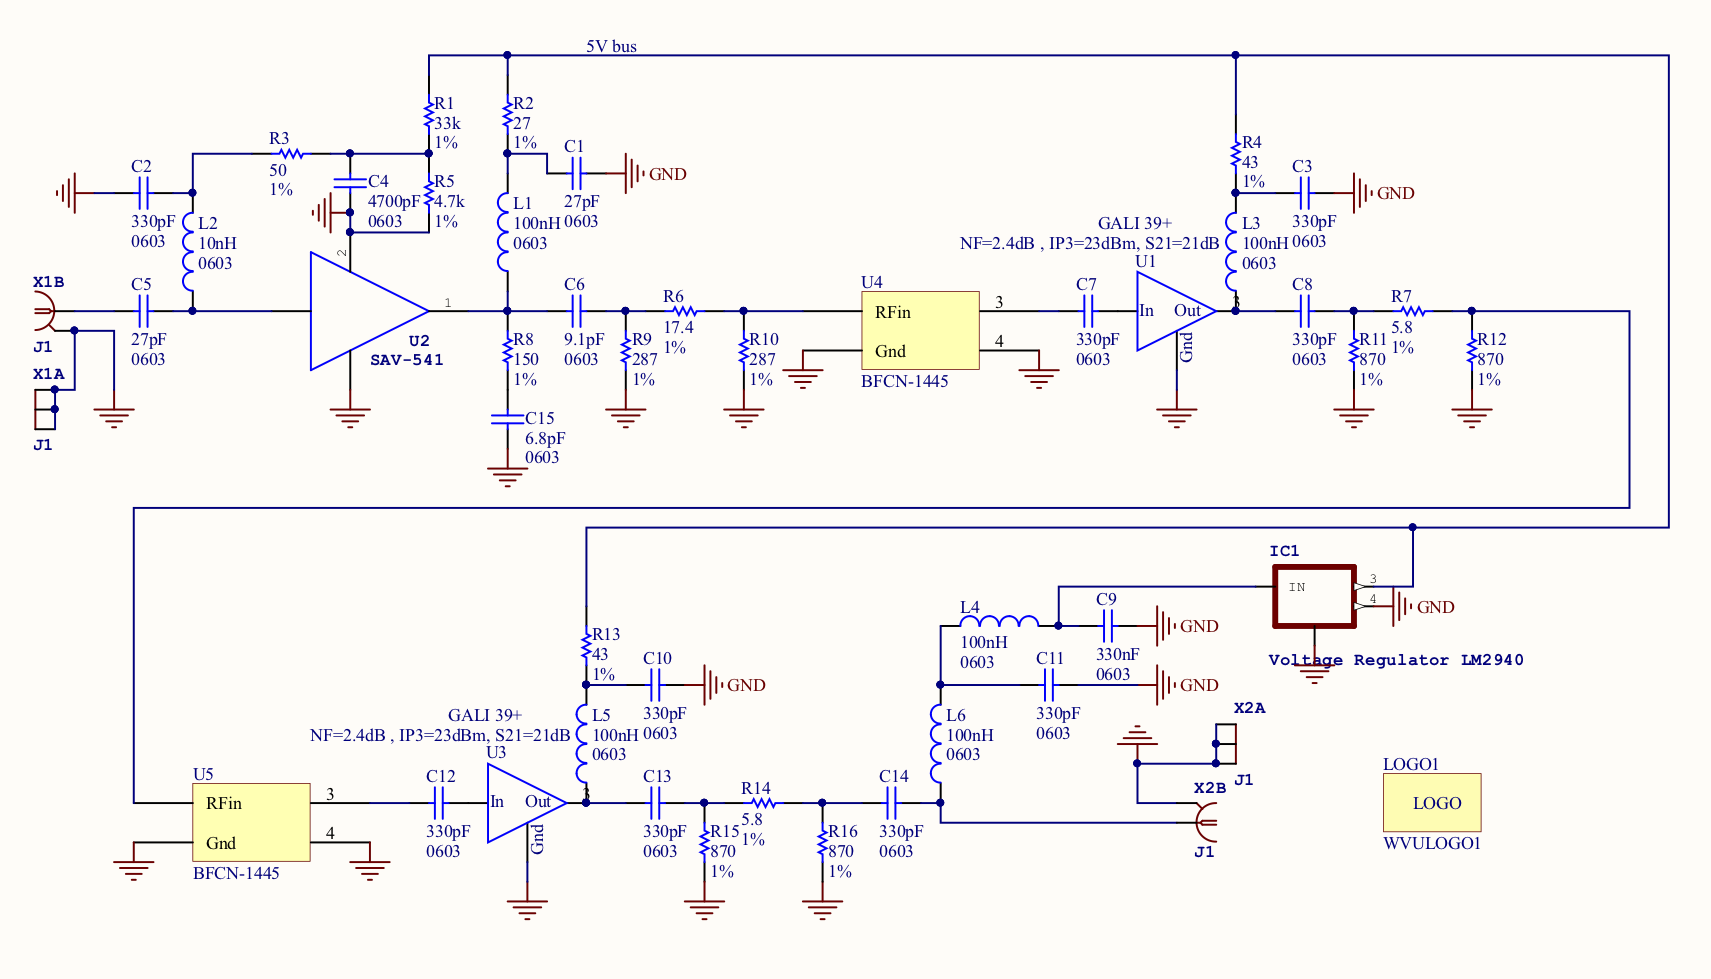
\includegraphics[width=.9\paperwidth]{schematic.png}}
\caption{Schematic of the LNA circuit}
\label{fig:schematic}
\end{sidewaysfigure}

\begin{sidewaysfigure}[tbh] 
\centering
 \makebox[\textwidth]{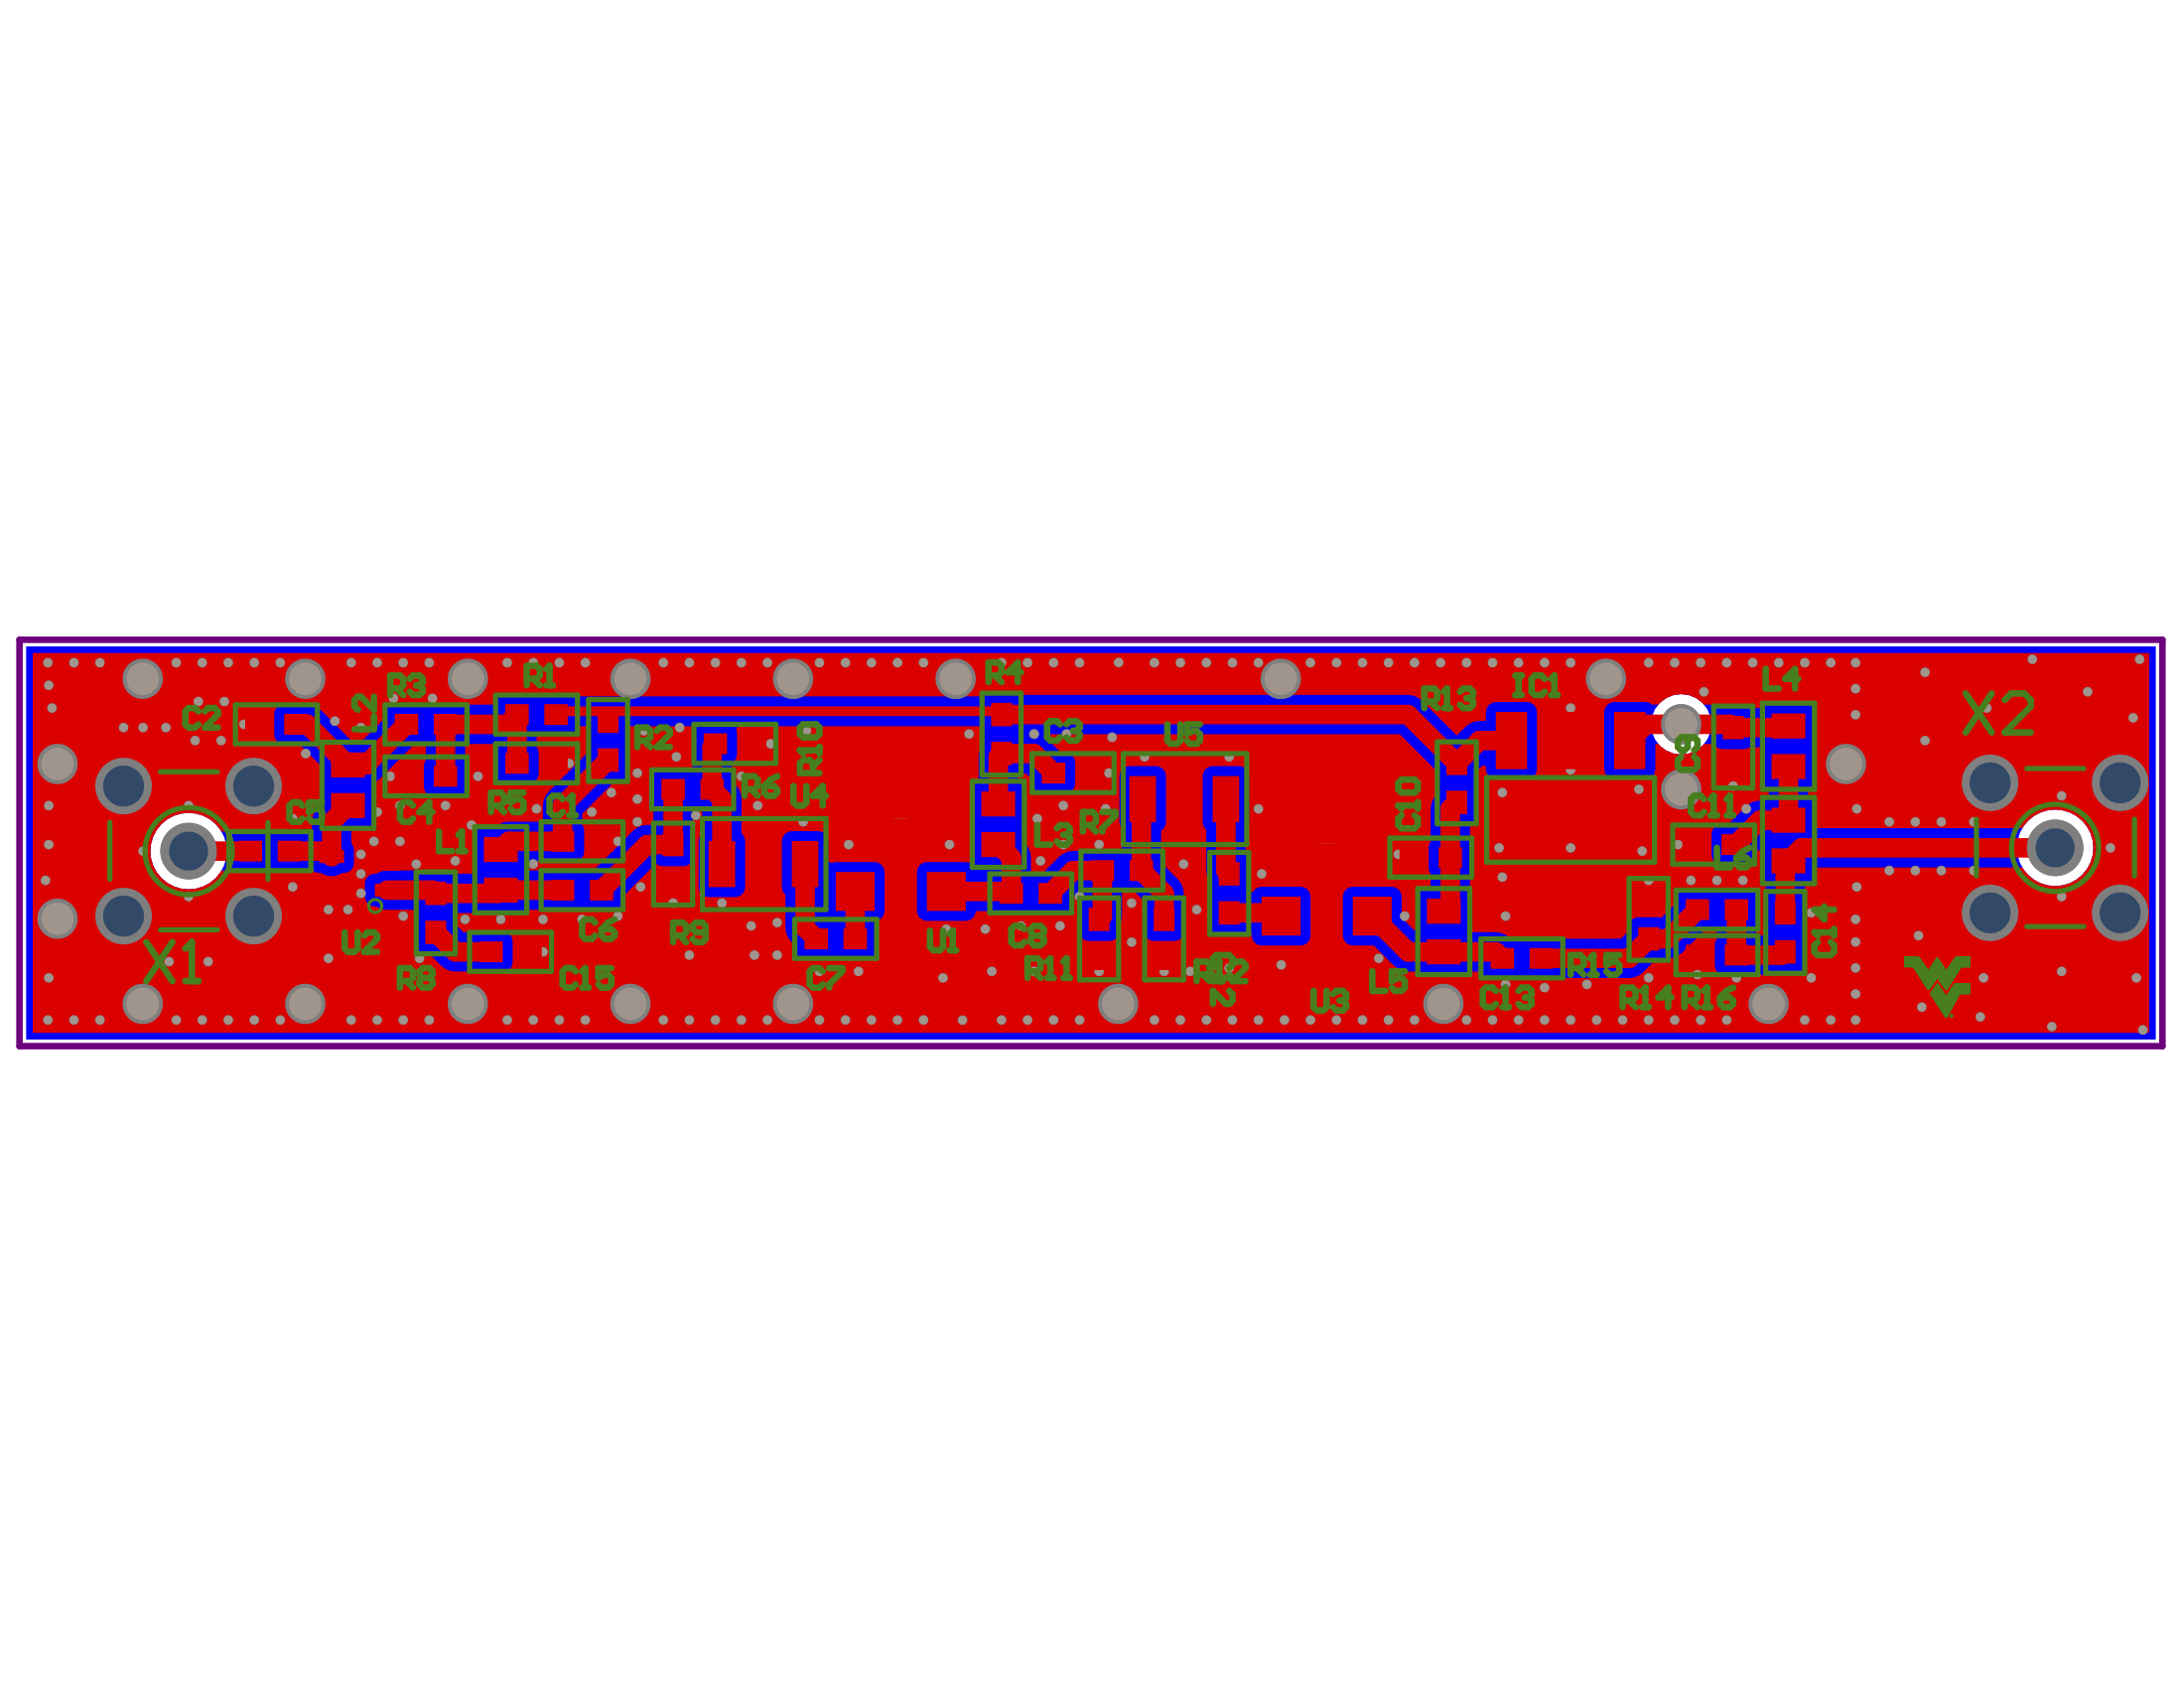
\includegraphics[width=.9\paperwidth]{layout.png}}
\caption{Schematic of the LNA circuit}
\label{fig:layout}
\end{sidewaysfigure}




\end{document}